\section{Overview}

Historically, the study of atmospheric-pressure plasmas (\acs{app}'s) is
indistinguishable from the study of plasmas as a whole. However, the detail of
the measurements and calculations associated with \acs{app}'s has been limited
by their complexity. From a computational perspective, the high pressure and
number of potential reactions present a difficult challenge. Likewise, the high
pressure can significantly complicate the data analysis for a number of plasma
diagnostics. Aside from the high pressures, the large electric fields, short
time scales, and general randomness of \acs{app}'s make even the most basic
observations a feat.

In the last several decades, some of this has begun to change. High-powered
computing has allowed simulations with remarkable detail. Similarly, advances in
technology has enabled plasma diagnostics in regimes that were experimentally
inaccessible. As a result, the body of knowledge regarding \acs{app}'s has
greatly increased. Sometimes, the motivation for this work is scientific
curiosity. More often, the study of \acs{app}'s has been driven by a broad range
of applications.

Among the first plasma applications were provided by \acs{app}'s: ozone
generation and lighting. Aside from these items, plasma welding, polymer
treatment, combustion, and plasma televisions have become widely accepted.
However, a large number of new applications may soon be added to this list,
including: treatment of tissue wounds, altering airflow over airfoils, and
destruction of industrial pollutants.

Unsurprisingly, each case has demands a different kind of plasma. The original
arc discharges were created between two graphite rods connected to immense
battery banks. In contrast, a modern research reactor studying plasma-assisted
combustion might use a fast-switching semiconductor circuit. Over the years,
several types of \acs{app}s have been developed for a variety of situations:
dielectric-barrier, corona, thermal arc, RF, microwave, pulsed, and more.

Within this group\footnote{The interested reader is referred to Starikovskaia's
review \cite{Starikovskaia2006} which provides a general overview of \acs{app}'s
in the context of plasma-assisted combustion}, the repetitively-pulsed
nanosecond discharge (\acs{rpnd}) has created considerable interest. Generally
speaking, a \acs{rpnd} is a plasma generated by a repetitive electrical pulse
applied between two electrodes. The pulse voltage if often $>1$ kV, lasts
anywhere from $<1$--$100$ ns, and is repeated over a thousand times each second.
The result is a wave of ionization (and light) which crosses from the powered
electrode to the grounded one.

A \acs{rpnd} can fill volumes of several liters with a relatively uniform
plasma. Though they can cause significant excitation of the background gas, they
generally produce very little heating (in some cases no more than a few kelvin
above room temperature). In addition, the excitation can be changed with
adjustments to the magnitude or duration of the electrical pulse. Each of these
characteristics are highly desirable in one or more of potential applications
for \acs{app}'s.

Given all of these promising properties, \acs{rpnd}'s have been the subject of
substantial study by several research groups. However, much of this work has
focused on the physics of \acs{rpnd}'s in air. Unfortunately, air's large number
of constituent elements can lead to notable complexity. In turn, this can
obscure some of the more fundamental questions relation to \acs{rpnd}'s: how do
they form, how is the energy distributed between excited particles, what kind of
spatial variation can be expected?

This paper details a study of each of these questions in a helium \acs{rpnd}.
Specifically, the densities of one particular excited atom are measured for a
variety of pressures and locations. This is complemented by measurements of the
light emissions for the same set of parameters. A simple model of a \acs{rpnd}
is used to predict several characteristics of the plasma based on the excited
state densities: electron density, electric field, and light emission. The
measured light emissions are interpreted to show how the energy is distributed
in the gas, and how it changes over time. Finally, they are compared with the
estimated light emissions to check the validity of several common assumptions.

The remainder of this chapter is comprised of a review of the associated
literature, as well as a discussion of basic discharge theory. Chapter
\ref{chp:exp} covers the experimental setup as well as some general observations
of the \acs{rpnd}. Next, the measurement of the excited state densities is
presented, followed by the chapter on the light emission measurements. Chapter
\ref{chp:model} explores the global model used to interpret the excited state
densities, as well as some supporting particle-in-cell simulations. Finally, the
paper concludes with a discussion of how the models and measurements impact the
present understanding of \acs{rpnd}'s.

\section{Literature Review}

Though \acs{rpnd}'s are very much a product of twentieth century research, they
are fundamentally similar to a number of other pulsed discharges such as
electrical sparks and lightning. Though Loeb united these disparate fields under
the title of ``ionizing waves of potential gradient'' in 1964 \cite{Loeb1965}
(we use the more familiar term, fast ionization waves), the underlying subjects
had been under study since the Greeks who generated sparks by rubbing together
amber and fur.

Despite these early observations, it was Leibniz in 1671 who first came to the
conclusion that sparks were an electrical phenomena \cite{Kryzhanovsky1989}.
Subsequently, Franklin's famous kite experiment led him to a similar conclusion
on the nature of lightning. Franklin was also involved in explaining the
principles of Leyden jars, develop by Musschenbroek. The Leyden jar was the
first reliable way to store electrical energy and proved a boon to later
research.

In 1835, Wheatstone made the first attempt to measure the speed of electricity
through a gas \cite{Wheatstone1835}. In his work, Wheatstone used a Leyden jar
connected to two metal spheres, separated by a small gap. Once the charge in the
jar reached a critical level, a spark would form in the gap. Figure
\ref{fig:wheatstone} shows the experimental sketch provided by Wheatstone.
\begin{figure}
  \centering
  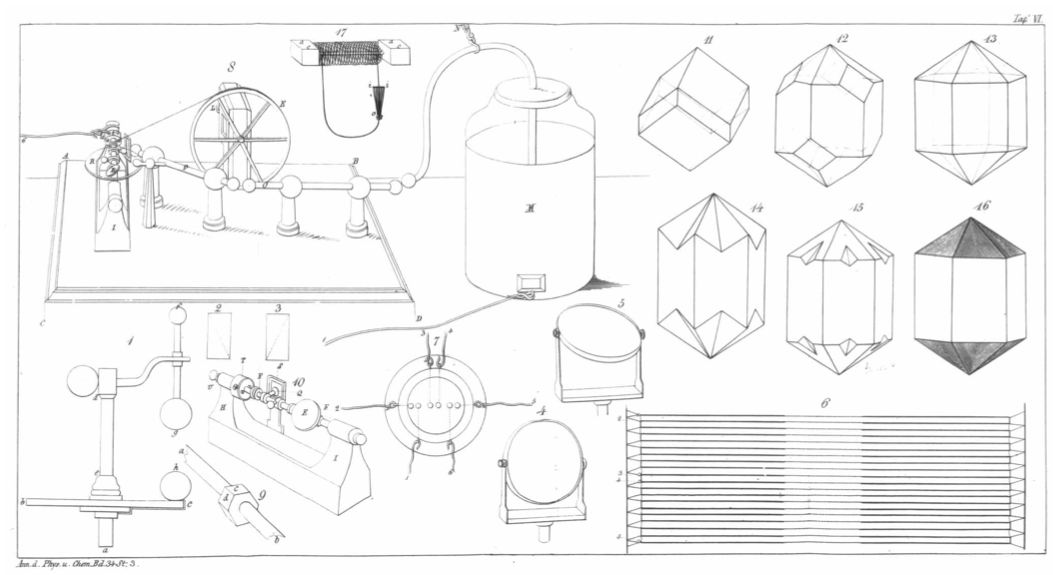
\includegraphics[width=4in]{chapters/introduction/figures/wheatstone.png}
  \caption{The experimental sketches of Wheatstone showing a traditional
  spark gap connected to a Leyden jar and electrostatic
generator.}\label{fig:wheatstone}
\end{figure}
Though the measurement is notable for its early date, it was later revisted with
much more accuracy by Thomson \cite{Thomson1893}. Perhaps the most important
outcome of Wheatstone's study was the observation by Zahn \cite{Zahn1879} that
the speed of the light was \emph{not} accompanied by a similar motion of the
emitting particles.

Thomson's work concerned both the speed and direction of light in a pulsed
discharge. Unlike Wheatstone's study, Thomson used an elongated tube, 15 m in
length, and 5 mm in diameter, upon which he drew a vacuum. The original sketch
of Thomson's discharge apparatus can be seen in figure \ref{fig:thomson}.
\begin{figure}
  \centering
  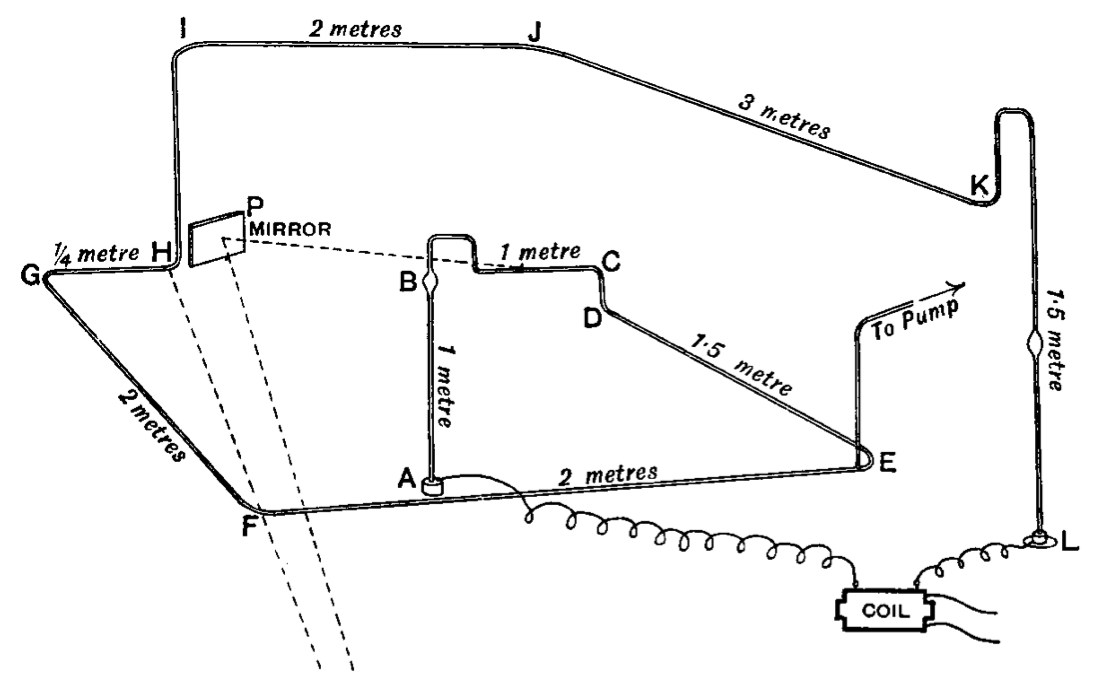
\includegraphics[width=4in]{chapters/introduction/figures/thomson.png}
  \caption{A sketch of J.J. Thomson's early experiments on fast ionization
  waves in long vacuum tubes.}\label{fig:thomson}
\end{figure}
Through a clever arrangement of mirrors, Thomson determined that the electricity
had a speed approaching $1\times10^{10}$ cm/s, and travelled from the anode to
the cathode.

It was later, in 1930, that Beams would determine that the wave always initiated
at the high voltage electrode, regardless of polarity \cite{Beams1930}. In
addition, Beams measured the current at the low potential electrode. He detected
a current pulse which did not appear until after the light had completely
crossed the gap. He came to the conclusion that the luminous front was likely
the result of a moving region of ionization.

As observed by Loeb \cite{Loeb1965}, there was a distinct set of researchers who
were attempting to study lightning. Despite Franklin's earlier realization that
lightning was an electrical phenomena, it was still unclear that it shared a
common origin with light pulses in rarefied gases. The endeavor was ambitious;
lightning was only predictable in the loosest sense of the word. In addition, it
was not clear what exactly could be measured.

In most cases, the study of lightning concentrated on time-resolved photography,
pioneered by Boys\footnote{In the same article, Boys anticipated a number of
other atmospheric physics studies by proposing that rockets be fired at 
thunderclouds. Unfortunately, he lived in a village of thatched houses and
could not conduct the experiment for fear of fire.}\cite{Boys1926}, and refined
by Schonland \cite{Schonland1935}. This technique was later adopted by Allibone
and Meek \cite{Allibone1938} to observe the evolution of a laboratory-generated
spark.

By 1935, fast ionization waves had been under study for nearly 50 years.
However, there was still no adequate explanation for the speed of the discharge.
Similarly, Beams' observation that the wave always travelled from the high
voltage to the low voltage electrode (regardless of polarity) could not be
accounted for. Based on observations made with fast pulses, Flegler and Raether
to developed a new theory of breakdown for sparks in air \cite{Flegler1936}
which was capable of, at least partly, explaining the fast ionization wave
phenomena. Independently, Loeb and Meek developed a similar theory in 1940
\cite{Loeb1940}.

\todo[inline]{Remember to include the laser dudes! Xenon lamps!}

\section{Basic Theory}

\subsection{Plasmas}

Most definitions of plasma use the phrase ``ionized gas.'' This implies that a
plasma is a gas with a finite amount of ionization. In the limit of no
ionization, the normal behavior of a gas should be recovered. Consequently, one
requirement for a plasma is that the electromagnetic effects of the charged
particles are the dominant interaction mechanism, compared to stochastic
effects. Quantitatively, this is written as
\begin{equation}
  \sqrt{n_\mathrm{e} e^2 / (\epsilon_0 m_\mathrm{e})} < \nu,
\end{equation}
where $n_\mathrm{e}$ is the electron density, $e$ is the fundamental charge,
$\epsilon_0$ is the permittivity of free space, $m_\mathrm{e}$ is the mass of an
electron, and $\nu$ is the electron-neutral collision frequency\footnote{A
similar oscillation frequency also exists for each electrically-charged species.
However, the electrons are the fastest to respond to electrical perturbations,
given their low mass. As a result, it is the electron-plasma frequency that is
used in this requirement.}. The term on the left is often denoted as
$\omega_mathrm{pe}$ and is referred to as the electron-plasma frequency.

However, this is not the only requirement for a gas to be considered a plasma.
There must also be a sufficient number of

\todo[inline]{requirements for a plasma}

Provided a sufficient number of particles, each species can be described by a
distribution function. This function, $f_\alpha(\vec{r}, \vec{v}, t)$, describes
the probability of finding a particle of species $\alpha$, at position
$\vec{r}$, with velocity $\vec{v}$, at time $t$. The distribution function for a
particle can be determined by the Vlasov-Fokker-Planck equation,
\begin{equation}\label{eq:vfp}
  \frac{\partial f_\alpha}{\partial t} + \vec{v}\cdot\nabla f_\alpha +
  q \left(\vec{E} + \vec{v}\times\vec{B}\right) \cdot \nabla_\mathrm{v} f_\alpha =
  \left( \frac{\partial f_\alpha}{\partial t}\right)_\mathrm{coll}.
\end{equation}
In essence, this is the Boltzmann equation from statistical mechanics, however
it now includes several changes. Vlasov replaced the original force term with
the Lorentz equation, and Fokker and Planck introduced the collision operator on
the right-hand side. This is coupled with Maxwell's equations for a solution of
the electric and magnetic fields in the plasma.

Unfortunately, depending on the collision operator, the Vlasov-Fokker-Planck
equation is a seven-dimension integro-differential equation which is notoriously
difficult to solve in anything but the most trivial of cases. As a result, most
plasma models use various moments of equation \ref{vfp} where the velocity
dependence has been integrated out. Each of these moments depends on a higher
one, thus it is necessary to truncate the moments at some point. It is common to
stop with the third moment which results in equations for: continuity of
density, conservation of moment, and conservation of energy,
\begin{gather}
  \

\subsection{Fast Ionization Waves}

\subsection{Atomic Spectroscopy}


